\section{\textsc{Schneller Gurkensalat mit saurer Sahne und Dill}}

\subsection*{Zutaten für 2 Portionen:}

\begin{tabular}{p{7.5cm} p{7.5cm}}
	& \\
	1 Salatgurke & 1 Becher Saure Sahne \\
	1 TL Gehackter Dill & Salz, Pfeffer
\end{tabular}

\subsection*{Serviervorschlag:}

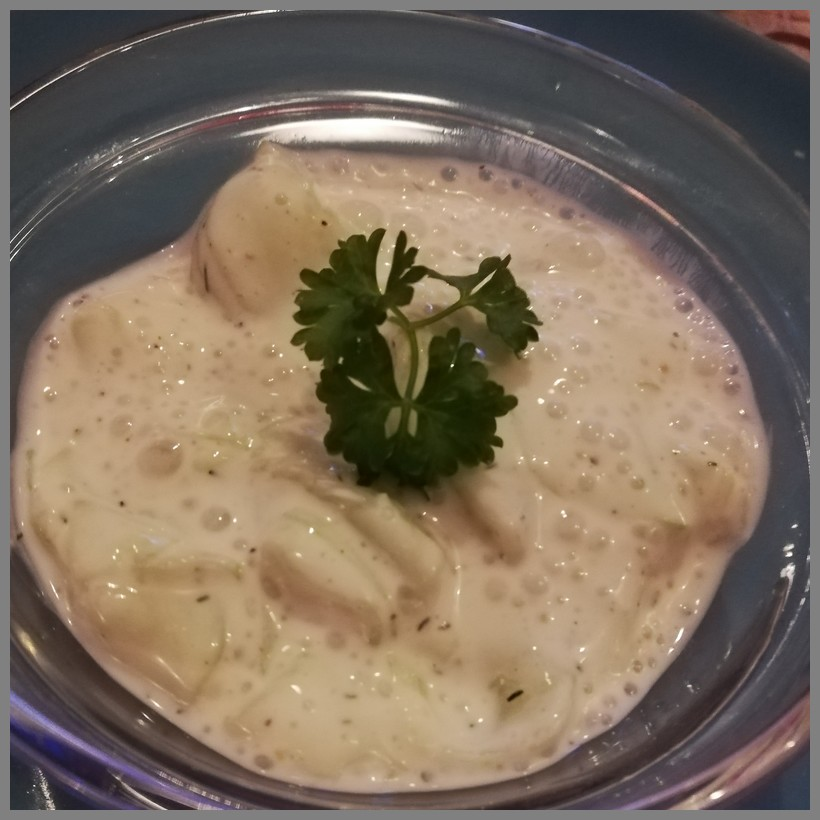
\includegraphics[width=\textwidth]{img/schneller_gurkensalat.jpg} \cite{gurkensalatdill}

\subsection*{So geht's:}

\begin{tabular}{p{15cm}}
	\\
  Die Gurke in dünne Scheiben schneiden, oder mit einer Küchenreibe reiben.\\
  Zusammen mit der sauren Sahne in eine Schüssel geben.\\
  Mit Salz und Pfeffer abschmecken.\\
  Frisch und gekühlt servieren.
\end{tabular}
